\documentclass[]{report}

\usepackage{fullpage}
\usepackage{graphicx}
\setlength\parindent{0pt}

% Title Page
\title{EVCO Open Assessment}
\author{Y6375144}


\begin{document}
\maketitle

\chapter{Introduction}

\section{Genetic Algorithms}

For some problems it can be difficult to find an optimal solution. This is because the search space grows at a much faster rate (exponentially, for example) than the input space. The Travelling Salesperson problem is a perfect example of this - for a search space with $n$ cities, there are $n!$ paths that the salesperson could take.\\

Evolutionary algorithms do not present a solution to this problem. However, by taking inspiration from biological evolution, they do offer an alternative approach that will often lead to a `good-enough' solution in a much more reasonable number of calculations. \\

Genetic algorithms are a type of evolutionary algorithm that typically represent population members (i.e. candidate solutions) in bitstrings. The population of strings is repeatedly updated through the following process:

\begin{enumerate}
	\item Select - A number of the existing population members are selected to continue through to the next round. Typically these would be the fittest members in the current population.
	\item Crossover - To generate new population members, existing ones are created by crossing two (or more) population members over. See figure \ref{crossoverFigure} for a visual representation.
	\item Mutate - The population is mutated at random. This typically involves passing over every bit in a string, and with a random probability flipping the bit from a 0 to a 1 (or vice versa).
	\item Evaluate - A fitness function is run on each member of the population, giving an indicator of how `good' a solution is.
\end{enumerate}

Genetic algorithms hold much potential, but in order to get the most from them you must carefully choose your representation and parameters. The representation is the bit string typically, but it can also take other forms. There are many parameters that can be fine tuned, such as the number of offspring to breed (at the crossover stage), or the type of crossover to perform.

\begin{figure}[h!]
	\begin{center}
		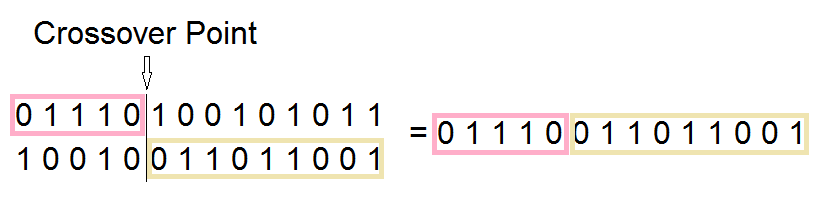
\includegraphics[scale=0.4]{figures/crossover.png}
		\caption{The child is made up of the top row (which represents the first parent) until the crossover point, where it then takes from the bottom row (the second parent).}
		\label{crossoverFigure}
	\end{center}
\end{figure}

\section{The Problem}

Morpion Solitare is a one player game that is typically played on grid paper. To start, a cross shape is drawn in the centre of the page (as shown in figure \ref{morpionSolitare}). On each turn the player must add one cross that creates a line of five crosses either vertically, horizontally or diagonally. The lines may intersect, and in this particular variant the lines may also overlap (it could be argued that this makes the game easier). Figure \ref{morpionSolitare} shows a possible first three moves. Finishing at this stage would give an overall score of 3, as 3 lines of 5 crosses have been formed.\\

\begin{figure}
	\centering
	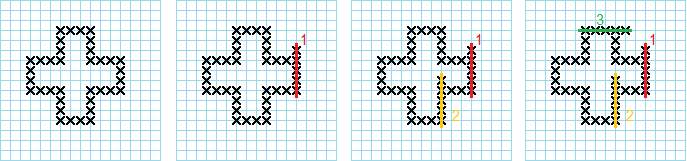
\includegraphics[width=\textwidth]{figures/combinedthreemoves.png}
	\caption{The initial state of the game on the left, and from left to right the first three moves are shown. The lines don't have to be numbered, but for clarity they are here.}
	\label{morpionSolitare}
\end{figure}

In this report I will detail my investigation into obtaining a high score through the use of a genetic algorithm. Working out the fitness of a population would be a tedious process if I have to take each population member and draw out its game from scratch. Thankfully that is not necessary as I have been provided with a computerised version of the game that is slightly faster.\\

When designing my genetic algorithm I will have to consider the format that the digital version takes its input by. The program represents positions on the grid by their $(x, y)$ co-ordinate positions, where $(0, 0)$ is the bottom left of the grid. For each move, four parameters must be passed into the program in the format $x_1 y_1 x_2 y_2$, where $(x_1, y_1)$ is the position of one end of the line to draw, and $(x_2, y_2)$ is the other end of that line. For the game shown in figure \ref{morpionSolitare}, the input would be:

\begin{verbatim}
	linuxMsolitare.exe 12 11 12 7 9 9 9 4 6 13 10 13
\end{verbatim}

The program accepts a maximum of 2000 inputs, or 500 moves. Given that the current best known solution is 178 \cite{morpionRecord}, this is unlikely going to be a problem. One potential problem is that to evaluate a population of size $n$, the application will need to be called $n$ times. Even with a decent processor, this could be a slow task for any sizeable population. Also, if a representation is chosen that doesn't directly map to the program's inputs is chosen, then each population member's representation will have to be converted to the correct format before the program can even be called. Again, this could be time consuming, but solutions to these problems will be considered in the next section.


\chapter{The Solution}

\section{Representation}

The standard genotype in a genetic algorithm is a bit-string. Studies have shown that in a lot of cases the algorithm will perform better when a bit string is used \cite{something}, although other studies suggest that this is not necessarily the case \cite{somethingElse}.\\

I will now discuss possible representations, and then explain my choice of representation.

\subsection{Gray Code Bit-string}

Binary bit-strings are not ideal for a genetic algorithm as a single bit flip during the mutation stage can cause the number to change a lot. Consider the bit string $10010110$ that represents the 8 bit unsigned integer 150. During mutation, if just the first bit is flipped, the string becomes $00010110$ and now represents 22. If the search space is a 256x256 grid, and that integer represents one co-ordinate, then 150 to 22 is a large jump. It would be more useful if the co-ordinate changed by just a small amount. If we wanted to change to 149 ($10010101$), two bit flips are required. \\

One solution to this is to use Gray code. This is a bit-string where each consecutive value differs by only one bit. In Gray code, $11011101$ represents 150, and $11011111$ represents 149. That's just a single bit flip, making Gray code ideal for genetic algorithms. \\

There are now a few possible options for how Gray code could be used to represent an individual move, and then a series of moves. The first option is to represent the co-ordinates as they are passed into the program in Gray code (remember that a move is passed in to the program as $x_1 y_1 x_2 y_2$). The grid 40x40, so ($\log _2 40 = 5.32$) 6 bits would be required to represent each co-ordinate. Each move would use 24 bits, and if the maximum number of moves is played each time (500), then 12000 bits or 1500 bytes will be required for each population member. If we have a population size of 5000, then the total required space will be 7.15MB.  \\

The second option is to store each move as a combination of (co-ordinate, direction), where co-ordinate is the new cross to draw on the board, and direction is the direction of the line. So ((20, 20), left) would mean draw a cross at position (20, 20), and draw left. This would then be translated into the program's input format $x_1 y_1 x_2 y_2$ to be 20 20 15 20.

\section{Selection}

\section{Crossover}

\section{Mutation}

\chapter{The Results}

\section{Conclusion}

\bibliography{bibliography}

\end{document}          
